
\chapter{Background}

We present here an overview of mechanisms and terminology used in both \xclaim and Zcash.
This section is not meant to be an in-depth examination of these systems, but merely to provide a basic understanding of the components therein, most importantly of those central to \zclaim.
For more material on the subjects, we refer the reader to the \xclaim research paper~\cite{zamyatin2019xclaim}, the original Zerocash paper~\cite{sasson2014zerocash,sasson2014zerocash_ext}, of which Zcash is an implementation, and the Zcash Protocol Specification (for the Sapling upgrade in specific, for which \zclaim has been designed)~\cite{hopwood2016zcash}.


\section{XCLAIM}
\label{sec:xclaim}

\xclaim is a generic passive-mode interoperability framework for cross-chain exchanges using \cbas.
It leverages smart contract logic, a dynamic set of economically incentivised, trustless intermediaries and cross-chain state verification to achieve decentralised asset interoperability.

\subsection{Setup}

In simple terms, \xclaim allows users to create \cbas on an \emph{issuing chain} $I$ backed by funds on a \emph{backing chain} $B$, and to redeem them again for backing currency at any moment.
The \emph{backing currency} on $B$ is denoted by $b$, the \emph{native currency} on $I$ by $i$ and the issued \cbas by $i(b)$.
In a slight abuse of notation, $b$, $i(b)$ and $i$ may also refer to quantities in these currencies where appropriate. $|x|$ denotes the monetary value of an amount of currency $x$.

The requirements on blockchains $B$ and $I$ are defined formally in~\cite[Section VI-B]{zamyatin2019xclaim}, but for the purpose of this review, we may assume that $I$ may be any smart-contract capable blockchain while all blockchains qualify as $B$.

Following actors take an active role in the protocol:
\begin{itemize}
    \item \textbf{Requesters} lock $b$ on $B$ to request the corresponding amount of $i(b)$ on $I$.
    \item \textbf{Redeemers} destroy $i(b)$ on $I$ to request the corresponding amount of $b$ on $B$.
    The redeemer of a certain amount of funds is not necessarily the same entity as their requester.
    \item \textbf{Vaults} are the non-trusted intermediaries that act as custodians, safekeep locked funds on $B$ and are liable for fulfilling redeem requests of $i(b)$ for $b$ on $B$.
    Anyone can take on the role of a vault by locking some collateral in $i$ and registering as a vault.
    Vaults are incentivised by fees they derive from transactions in which they take part.
    In case of misbehaviour, they face \emph{slashing}, which means partial or total liquidation of their collateral.
    \item The \textbf{issuing Smart Contract} (\textsf{iSC}) is a public smart contract responsible for managing the correct issuing of $i(b)$ on $I$ and for ensuring the correct behaviour of vaults.
    It maintains a public list of vaults along with the amount of collateral they have locked, their identities on $B$ and the amount of $b$ that they hold.
    
    The \textsf{iSC} verifies transactions on $B$ through a chain relay~\cite{Back2014sidechains,buterin2016interop}, which stores and maintains block headers from blocks in $B$ on $I$.
    It is assumed each block header contains the root of a Merkle tree containing all transactions or transaction identifiers for that block.
    The chain relay allows the \textsf{iSC} to verify that a transaction has been included on $B$ if a Merkle path from the transaction to this root is provided.
    We call this an \emph{inclusion proof}.
    Furthermore, the chain relay is able to verify if consensus has been reached on a certain block in $B$.
    How this is achieved depends on the consensus mechanism used in $B$.
\end{itemize}

\subsection{Blockchain model and assumptions}
\label{sec:blockchain_model}

\xclaim assumes that the consensus mechanisms employed by $B$ and $I$ cannot be corrupted by an adversary, in order to ensure safety and liveness of the underlying blockchains.
The specific assumptions depend on the consensus mechanism of the respective blockchain.
For example, if $B$ or $I$ employ the Nakamoto consensus mechanism, such as Bitcoin~\cite{nakamoto2008bitcoin} or Ethereum~\cite{wood2014ethereum}, it is assumed that the computational power of an adversary is limited by $\alpha < 33\%$.
For Proof-of-Stake mechanisms with similar Byzantine fault tolerance, such as the upcoming Ethereum 2.0 upgrade~\cite{Ethereum2.0pos} or~\cite{buchman2016tendermint,Kiayias2017ouroboros}, it is assumed $f<n/3$, where $n$ is the total number of consensus participants.
Note that other Proof-of-Stake systems, such as~\cite{tezos2014whitepaper}, may assign voting power based on the staked amount or other criteria instead of per participant.
In this case, it would be accurate to define $f$ as the fraction of voting power held by the adversary.

This guarantees that the fraction of maliciously generated blocks are upper bounded by $\frac{f}{n-f}$ and hence that the probability of a blockchain reorganisation drops exponentially with security parameter $k \in \N$. $k$ denotes the block depth, i.e., the position of a block relative to the tip of the blockchain. A transaction is considered \textcquote[3]{zamyatin2019xclaim}{\emph{securely} included in the underlying blockchain if, given the current blockchain head at position $h \in \N$, the transaction is included in a block at position $j \in \N$, such that $h-j \geq k$}. The security parameter $k$ is denoted $k^B$ for $B$ and $k^I$ for $I$.

$\Delta^I$ and $\Delta^B$ denote the delay from transaction broadcast to its secure inclusion on blockchains $I$ and $B$, respectively.
$\Delta_{submit}$ is the delay from block creation on $B$ to the time a transaction submitting its block header to the chain relay is broadcast.

To manage exchange rate fluctuations between $b$ and $i$, \xclaim assumes an oracle $\mathcal{O}$ provides the \textsf{iSC} with the exchange rate $\epsilon_{(i,b)} \in \R_{\geq 0}$ such that $1\, i = \epsilon_{(i,b)} \, b$.

For the underlying network, it is assumed \textcquote[3]{zamyatin2019xclaim}{(i) honest nodes are well connected and (ii) communication channels between these nodes are (semi-)\-synchronous. Specifically, transactions broadcast by users are received by (honest) consensus participants within a known maximum delay $\Delta_{tx}$}.

\subsection{System goals}
\label{sec:xclaim_goals}

\xclaim achieves a number of security properties, defined as follows in~\cite[Section III-E]{zamyatin2019xclaim}:
\begin{itemize}
    \item \textbf{Auditability.} Any user with read access to blockchain $B$ and $I$ can audit the operation of \xclaim and detect protocol failures.
    \item \textbf{Consistency.} No \cba units $i(b)$ can be issued without the equivalent amount of backing currency $b$ being locked, i.e., that $|b| = |i(b)|$.
    \item \textbf{Redeemability.} Any user can redeem \cbas $i(b)$ for backing currency $b$ on $B$, or be reimbursed with equivalent economic value on $I$.
    \item \textbf{Liveness.} Any user in \xclaim can issue, transfer and swap \cbas without requiring a third party, i.e., liveness relies only on the secure operation of $B$ and $I$.
    \item \textbf{Atomic Swaps.} Users can atomically swap \xclaim \cbas against other assets on $I$ or the native currency $i$.
\end{itemize}

\subsection{Protocols}

There are two main protocols in \xclaim: \emph{Issue}, allowing the creation of $i(b)$, and \emph{Redeem}, which involves \emph{burning} (destroying) $i(b)$ in exchange for $b$.
Besides, \xclaim defines two protocols \emph{Transfer} and \emph{Swap}, outlining the transfer of $i(b)$ among participants on $I$ and its exchange for $i$, respectively, with which we do not concern ourselves here.
A diagram from the original \xclaim paper showcasing the different stages in these protocols can be seen on \cref{fig:xclaim_protocol}.

\begin{figure}
\centering
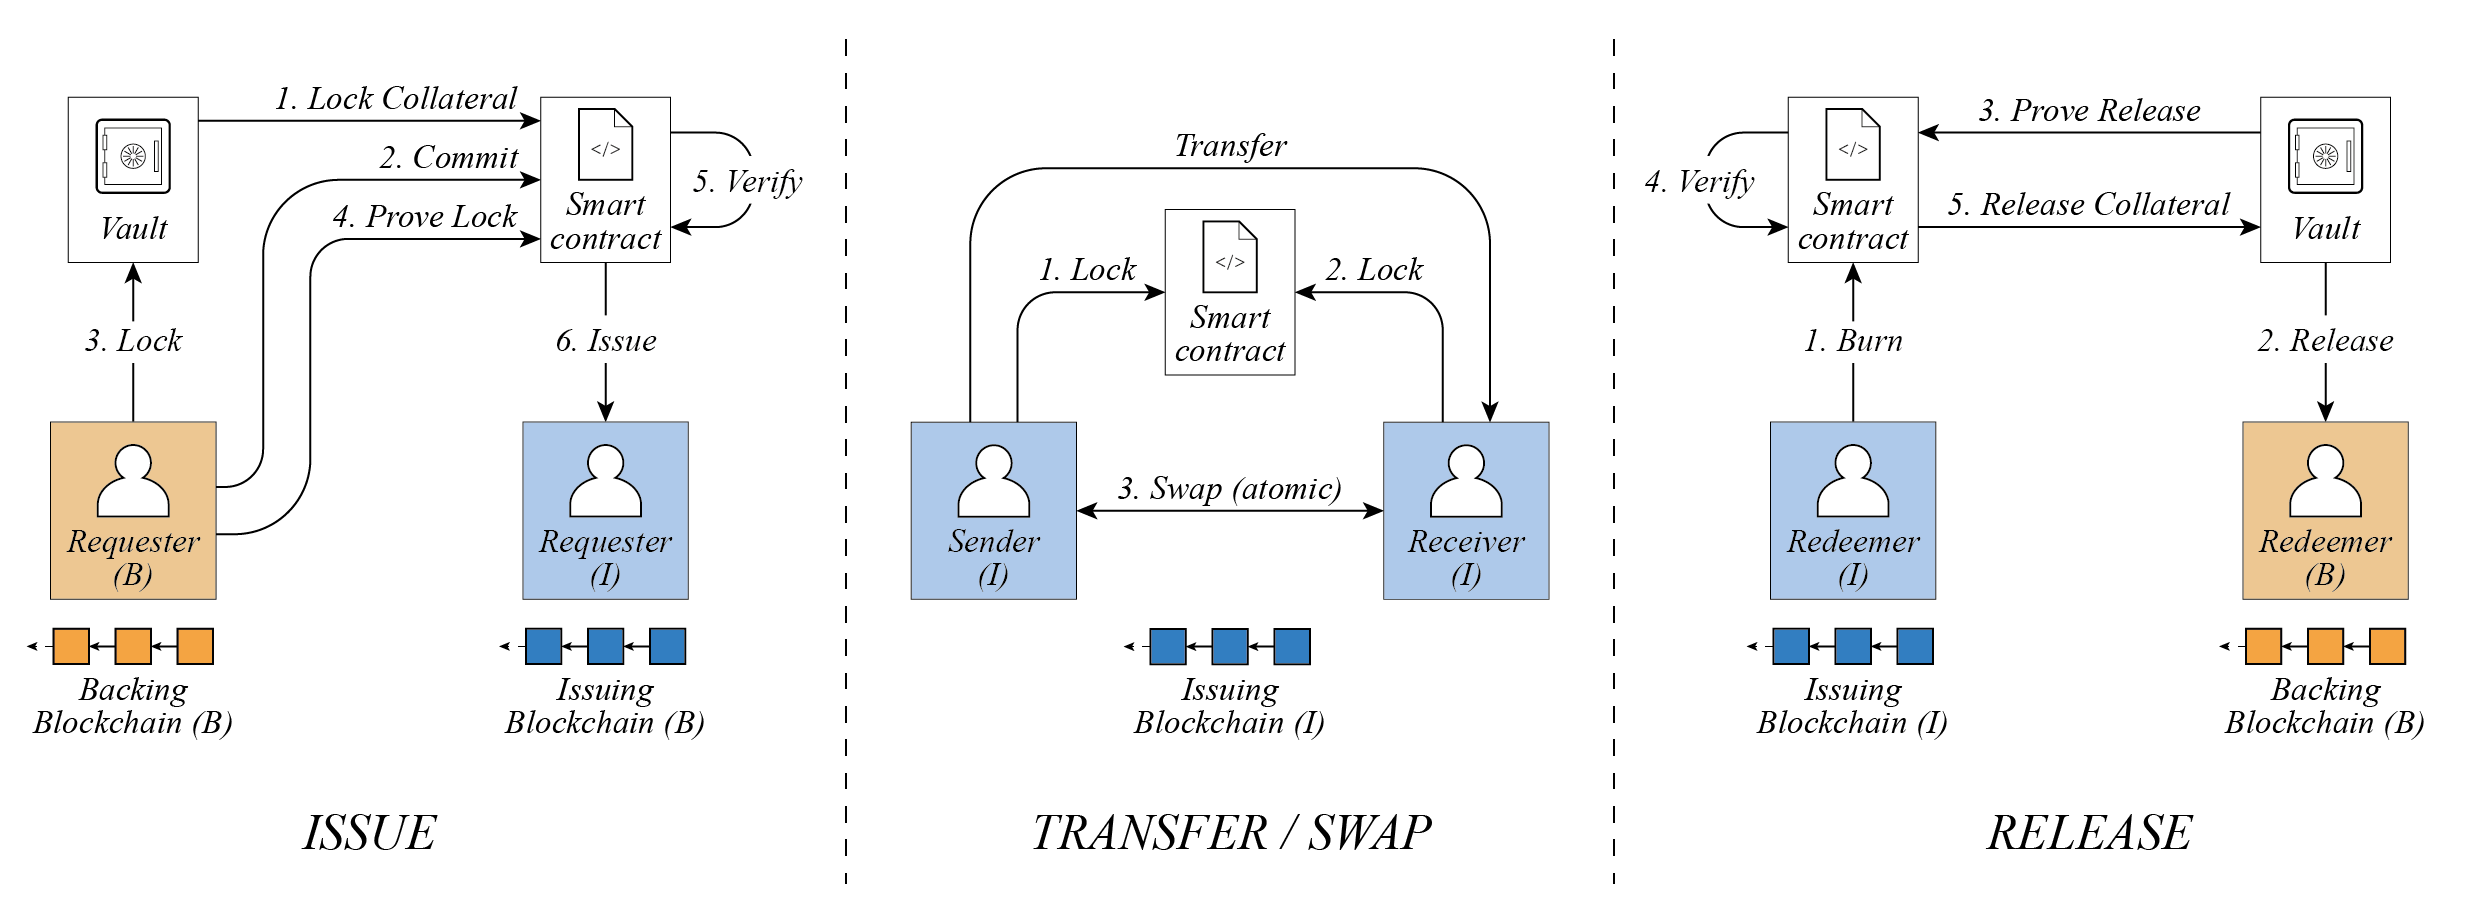
\includegraphics[width=1.0\textwidth]{img/xclaim.png}
\caption{Overview of the different protocols in \xclaim.}
\label{fig:xclaim_protocol}
\end{figure}

\emph{Issue} and \emph{Redeem} are defined as follows:

\textbf{Protocol: Issue.} Alice (requester) locks units of $b$ with a vault on $B$ to create $i(b)$ on $I$:
\begin{enumerate}
    \item \emph{Setup.}
    The vault registers with the \textsf{iSC} and locks $i_{col}$ units of collateral, where it must hold that
    \begin{equation}\label{eq:collateral}
        i_{col} \geq b_{lock} \cdot r_{col} \cdot \epsilon_{(i,b)} \geq b_{lock}
    \end{equation}
    where $b_{lock}$ is the amount of funds that Alice will lock, $r_{col}$ is an over-collateralisation factor in order to account for future exchange rate fluctuations, and $\epsilon_{(i,b)}$ is the exchange rate at the time Alice commits to locking funds (next step).
    
    Alice verifies the \textsf{iSC} smart contract is available on chain $I$, i.e., the issuing blockchain, and both chooses a vault that satisfies \cref{eq:collateral} and learns its identity on $B$ through the \textsf{iSC}.
    
    \item \emph{Commit.}
    Alice generates a new public/private key pair on $I$ and commits to locking funds $b_{lock}$ with the vault by providing a small amount of collateral to the \textsf{iSC}.
    This is in order to avoid \emph{griefing} attacks in which Alice repeatedly commits to issuing with the vault without actually doing so.
    The collateral is refunded to Alice when she issues the funds.
    
    In future issue requests, the vault will only be able to issue $i(b) = \frac{i_{col}}{r_{col} \cdot \epsilon_{(i,b)}} - b_{lock}$ and the amount of collateral backing $b_{lock}$ is said to be \emph{blocked}.
    If Alice fails to complete \emph{Issue}, however, this collateral becomes \emph{free} again.
    
    \item \emph{Lock.}
    Alice locks funds $b_{lock}$ with the vault on $B$ in a publicly verifiable manner, i.e., by sending $b_{lock}$ to the vault.
    As part of locking these funds with the vault, Alice also specifies where the to-be-generated $i(b)_{issue}$ should be sent, i.e., Alice associates her public key on $I$ with the transfer of $b_{lock}$ to the vault.
    
    \item \emph{Create.} Alice proves to the \textsf{iSC} that the funds were locked by providing an inclusion proof for her transaction to the chain relay.
    The \textsf{iSC} verifies that the transaction is correct and consensus has been reached on the given block, then creates and sends $i(b)_{issue}$ to Alice's public key in the transaction such that $|i(b)_{issue}| = |b_{lock}|$.
\end{enumerate}

\textbf{Protocol: Redeem.} Dave (redeemer) locks $i(b)$ with the \textsf{iSC} on $I$ to receive $b$ from a vault on $B$; the $i(b)$ are then destroyed:
\begin{enumerate}
    \item \emph{Setup.}
    Dave creates a new public/private key pair on $B$ and chooses a vault that can release the amount of funds $b_{release}$ he wishes to redeem, i.e.\ holds $b$ such that $b_{vault} \geq b_{release}$, through the \textsf{iSC}.
    
    \item \emph{Lock.}
    Next, Dave locks $i(b)_{burn}$ with the \textsf{iSC} on $I$ and requests their redemption.
    Thereby, Dave also specifies the vault he has chosen to release his funds and his public key on $B$ as the target for the redeem.
    
    \item \emph{Release.}
    The vault witnesses the locking and redemption request of $i(b)_{burn}$ on $I$ and releases funds $b_{release}$ to Dave’s specified public key on $B$, such that $|b_{release}| = |i(b)_{burn}|$.
    
    \item \emph{Burn.}
    Finally, the vault confirms with the \textsf{iSC} that $b_{release}$ was redeemed on $B$ by providing an inclusion proof for the release transaction, and the \textsf{iSC} burns the locked $i(b)_{burn}$ on $I$.
    The amount of the vault's collateral backing $b_{release}$ (see \emph{Issue} protocol) becomes free again.
    
    Alternatively, if the vault fails to confirm the release, it is slashed and Dave is compensated in $i$ from the vault's collateral such that $|b_{release}| = |i_{slash}|$.
\end{enumerate}

Based on $\Delta_{submit}$, $\Delta^I$ and $\Delta^B$, sensible timeouts for the different stages of these protocols are suggested.
A formal specification of all protocols in \xclaim can be found in~\cite[Section VI-A]{zamyatin2019xclaim}.

Finally, \xclaim employs automatic liquidation to address exchange rate fluctuations outside of the over-collateralisation factor.
That is, if a vault's observed collateral rate $r_{col}^* = \frac{i_{col}}{r_{col} \cdot \epsilon_{(i,b)}}$ is critically close to the lower bound of 1.0, the \textsf{iSC} allows anyone to redeem their $i(b)$ for $i$ at a markup until the vault's entire collateral has been sold.

\section{ZCash}
\label{sec:zcash}

Zcash is an implementation of the Decentralized Anonymous Payment scheme Zerocash~\cite{sasson2014zerocash}.
It builds on Bitcoin's~\cite{nakamoto2008bitcoin} transparent payment scheme, adding a shielded payment scheme to it that leverages zero-knowledge succinct non-interactive arguments of knowledge (\emph{zk-SNARKs}) to enable private payments.

Although Bitcoin's payment scheme is an integral part of Zcash (in fact, as noted by \textcite{kappos2018anonymity}, over 85\% of all Zcash transactions up until January 2018 had taken place solely within Bitcoin's transparent payment scheme), this work focuses on bringing cross-chain interoperability to Zcash's shielded payment scheme.
\xclaim already defines an interoperability framework for transparent payment schemes such as Bitcoin, hence the contributions in this work may be thought of as supplementary to \xclaim's design in order to obtain a framework that covers all types of transactions in Zcash.

Therefore, after a brief explanation on how these two payment schemes coexist and interact in Zcash, the rest of this work will focus on Zcash's shielded payment scheme.

Transactions in Zcash can contain transparent inputs, outputs, and scripts, which all work as in Bitcoin, and shielded \emph{JoinSplit}, \emph{Spend} and \emph{Output descriptions}, which are the encodings of \emph{JoinSplit}, \emph{Spend} and \emph{Output transfers} in a transaction.
A transaction may combine transparent and shielded components such that value is moved from the \emph{transparent value pool} to the \emph{shielded value pool} or vice-versa.
This process is referred to as \emph{shielding} or \emph{deshielding}, respectively.

JoinSplit transfers were introduced in the original implementation of Zcash and are still supported in Sapling for backwards compatibility.
We choose not to support these and instead design \zclaim based on the Spend and Output transfers introduced in the Sapling upgrade, which offer a more flexible approach to shielded spending among other improvements not discussed here.

Spend and Output transfers are analogous to transparent inputs and outputs, respectively.
Each Spend transfer spends a shielded \emph{note}, and each Output transfer creates one.
A note represents that a value \val is spendable by the recipient who holds the \emph{spending key} corresponding to the destination \emph{shielded payment address}.
A note's sender, recipient and value are never revealed.

To each note there is a cryptographically associated \emph{note commitment}, which is added to the \emph{note commitment tree} when the note is created.
Only notes whose note commitment is in the note commitment tree can be spent.

When the note is spent, a unique \emph{nullifier} associated with that note must be revealed and is then added to the \emph{nullifier set}.
It is infeasible to compute the nullifier without the spending key\footnote{Technically, without the nullifier deriving key, which is derived from the spending key.} corresponding to the recipient's shielded payment address.
Only notes whose nullifier is not in the nullifier set can be spent.

The main premise of Zcash's shielded payment scheme is that when a note is spent, the spender only proves that its note commitment is in the note commitment tree, without revealing which one.
Revealing its nullifier also does not give away its note commitment.
This means that a spent note cannot be linked to the transaction in which it was created.

Spend and Output transfers both contain a \emph{value commitment} to the value of the note being spent or created.
Furthermore, they contain computationally sound zk-SNARKs proofs and signatures which prove that all of the following hold except with insignificant probability.

For Spend transfers:
\begin{itemize}
    \item the spender knows a note whose note commitment is in the note commitment tree;
    \item the revealed value commitment was derived from the value in the note;
    \item the spender knows the proof authorising key (which is again derived from the spending key, see \cref{sec:zcash_addr} for an overview of key components in Sapling and the relations between them) corresponding to the shielded payment address in the note;
    \item the revealed nullifier is computed correctly.
\end{itemize}

And for Output transfers:
\begin{itemize}
    \item the revealed note commitment is computed correctly;
    \item the revealed value commitment was derived from the value in the note used to generate the note commitment.
\end{itemize}

All Spend and Output transfers in a transaction, along with any transparent inputs and outputs, are checked to balance by verifying that the sum of all value commitments and of all transparent values is equal to zero.

\subsection{Commitment schemes}

A commitment scheme is a function that takes an input and a random \emph{commitment trapdoor}, and returns a \emph{commitment} to the input such that:
\begin{itemize}
    \item No information is revealed about it without the trapdoor (`hiding'),
    \item Given the trapdoor and input, the commitment can be verified to \emph{open} to that input and no other (`binding').
\end{itemize}

Commitment schemes are used to hide the value in Output and Spend transfers and to generate note commitments.
The precise definition can be found under~\cite[4.1.7]{hopwood2016zcash}.

\subsection{Addresses}\label{sec:zcash_addr}

A shielded payment address, which we may refer to simply as a \emph{payment address}, consists of a \emph{diversifier} \dvf and a \emph{transmission key} \pkd. 
This address is ultimately derived from a spending key as depicted in \cref{fig:zcash_addr}.

\begin{figure}
\centering
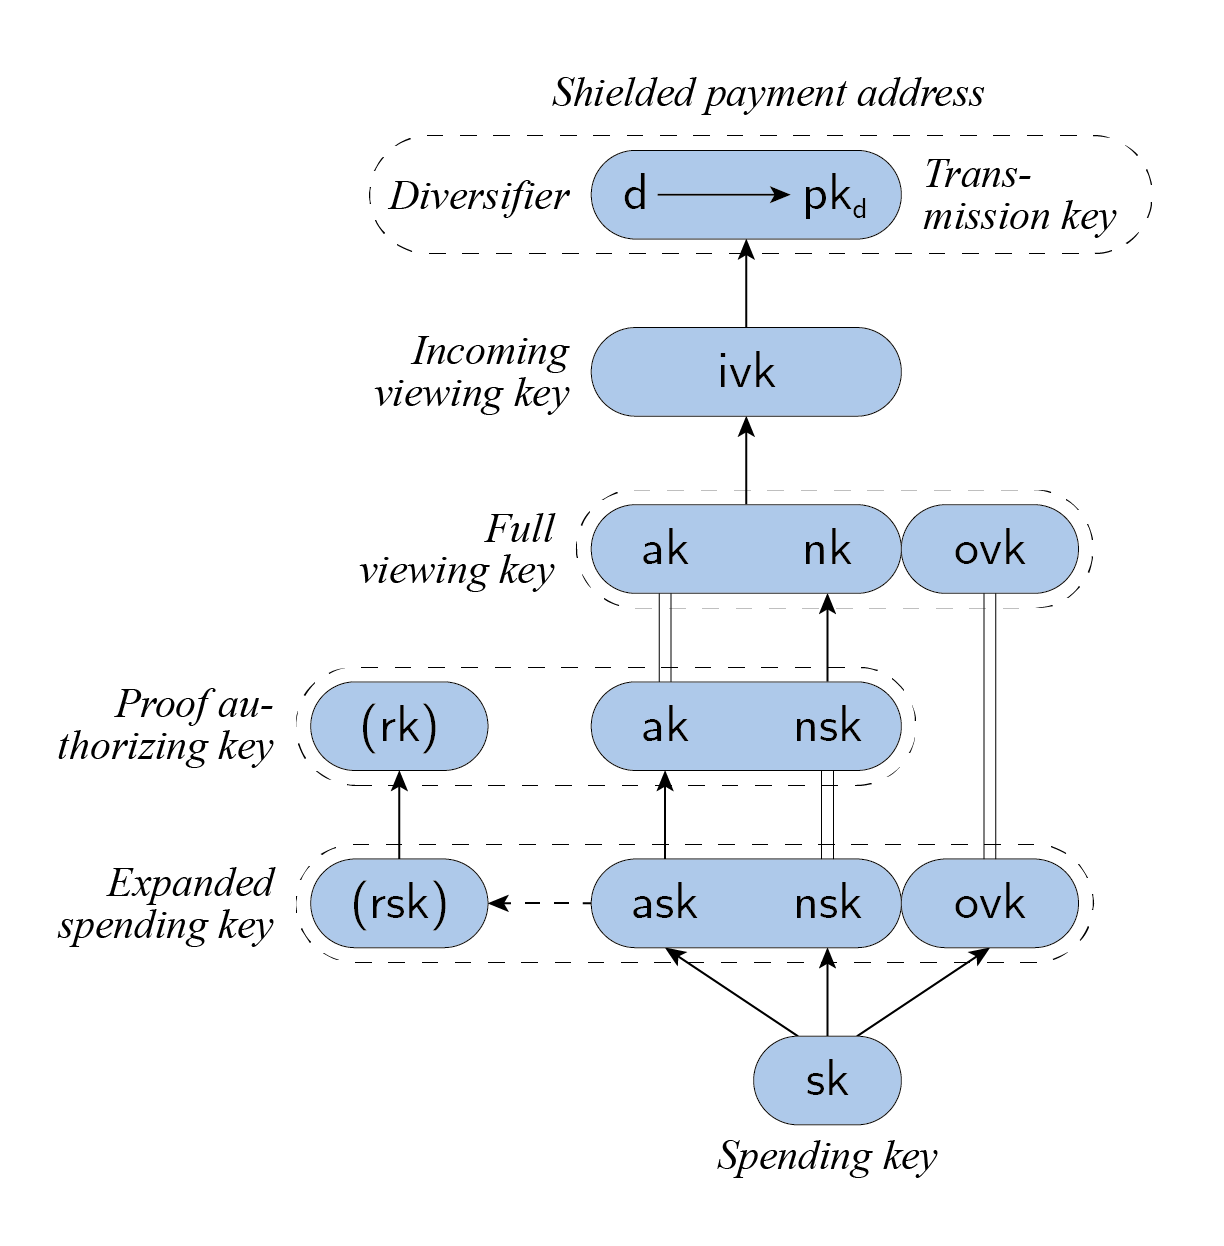
\includegraphics[width=0.6\textwidth]{img/zcash_addresses.png}
\caption[Sapling address components]{Sapling address components. Arrows signalise that a component is derived from another one. Double lines denote the same component.}\label{fig:zcash_addr}
\end{figure}

As for the intermediate components, the \emph{expanded spending key} is composed of a \emph{spend authorising key} \ask and a \emph{nullifier private key} \nsk, which are necessary to spend a note, and the outgoing viewing key \ovk, which allows a user to decrypt notes spent by themselves.
The \emph{proof authorising key} allows devices that are computationally or memory-limited to delegate the generation of the zk-SNARK proof in Spend transfers to a third party.
The key \rsk is used to sign transactions and is a re-randomisation of the spend authorising key, while \rk is the public key derived from it.

A \emph{full viewing key} allows users to decrypt notes sent and received by them.
Specifically, received notes can be decrypted using the \emph{incoming viewing key} \ivk derived from the \emph{nullifier deriving key} \nk and the (unnamed) \ak components of the full viewing key.
Spent notes can then be identified by using the nullifier deriving key to derive the nullifiers of received notes and checking for their existence in the nullifier set.
Together with the outgoing viewing key, this allows a user to decrypt all previous and future activity associated with the corresponding spending key.

See~\cite[Section 4.2.2]{hopwood2016zcash} for types and derivation methods of the different key components.

\subsection{Notes}

Notes are similar to Bitcoin's Unspent Transaction Outputs or UTXOs, with the difference that by definition only unspent transaction outputs are stored in the UTXO set in order to be spent at a later point without needing to scan the entire blockchain.
In Zcash, in contrast, all note commitments are stored in the note commitment tree, as it is not possible to tell an unspent note from a spent one.

A Sapling note \n is defined as the tuple
\[
    (\dvf : \B^{[\ld]},\, \pkd : \J ,\, \val : \{0\,..\,2^{\lval}-1\},\, \rcm : \{0\,..\,2^{\lscalar}-1\})
\]
where:
\begin{itemize}
  \item \dvf is the diversifier of the recipient's payment address.
  \item \pkd is the diversified transmission key of the recipient's payment address.
  \item \val is an integer representing the value of the note in \emph{zatoshi}, ZCash's smallest unit of currency. 1 zatoshi = $10^{-8}$ ZEC.
  \item \rcm is a random commitment trapdoor used to derive the note commitment for this note.
\end{itemize}

\medskip
The \emph{note plaintext} \np is the representation of a note in transactions, defined as
\[
    (\lby : \By, \dvf : \B^{[\ld]}, \val : \{0\,..\,2^{\lval}-1\}, \underline{\rcm} : \By^{32}, \memo : \By^{512})
\]
where \lby is always 0x01 for Sapling notes, and \memo may contain any additional information that the sender of the note wishes to transmit to the receiver.

The corresponding note commitment is calculated using \rcm as the trapdoor and the concatenation of the remaining values as the input value.

\subsection{Note commitment tree}

The note commitment tree is a Merkle tree of fixed depth.
Every node in this tree contains a hash computed from their children in the next layer, except for the outmost layer containing the note commitments.
The index of a note's commitment at this layer is called its \emph{note position}.
When a note is created, its commitment is added to the outmost layer as a new leaf and thus the value in all of the leaf's ancestors including the root changes.
A \emph{positioned note} refers then to the note along with its position in the note commitment tree.

Every transaction has an input and an output \emph{treestates}, which denote the state of the note commitment tree before and after adding any newly created notes.
A block's input and an output \emph{treestates} are defined as the output treestate of the last transaction in the preceding block and in that block, respectively.
An \emph{anchor} is the Merkle root of the note commitment tree in a given treestate.

Hash values are computed using a non-padded version of the SHA-256 hash function as defined in~\cite{nist2015shs}.

\subsection{Spend and Output descriptions}

A Spend transfer is encoded in transactions as a Spend description, which is defined as the tuple $(\cv, \rt, \nf, \rk, \pis, \sas)$, where:
\begin{itemize}
    \item \cv is the value commitment to the value of the input note.
    \item \rt is an anchor for the output treestate of a previous block.
    \item \nf is the note's nullifier.
    \item \rk is a randomized validating key derived from the spend authorisation key that should be used to validate \sas.
    \item \sas is a signature over the SIGHASH transaction hash as defined in~\cite{ZIP243}.
    This signature proves knowledge of the spending key and guarantees that this Spend transfer cannot be replayed in other transactions.
    \item \pis is a zk-SNARK proof for a Spend statement with primary input $(\cv, \rt, \nf, \rk)$, as defined in~\cite[Section 4.15.2]{hopwood2016zcash}.
\end{itemize}

On the other hand, an Output description consists of $(\cv, \cmu, \epk, \cenc, \cout,\allowbreak \pio)$, where:
\begin{itemize}
    \item \cv is the value commitment to the value of the output note.
    \item \cmu is an integer representation of the note commitment for the output note.
    \item \epk is an ephemeral key agreement public key, used to derive the key for encryption of the transmitted note ciphertext.
   \item \cenc is a ciphertext component containing the note plaintext, encrypted with a key agreement scheme using the private key \esk from which \epk was derived and the diversifed transmission key \pkd of the recipient.
   The recipient can decrypt this component using his incoming viewing key \ivk and \epk.
   \item \cout is a ciphertext component that allows the holder of an outgoing viewing key to recover \esk and \pkd, which can then be used to recover the note plaintext from \cenc.
   \item \pio is a zk-SNARK proof for an Output statement with primary input $(\cv, \cmu, \epk)$, as defined in~\cite[Section 4.15.3]{hopwood2016zcash}.
\end{itemize}

Observe that the ciphertext components \cenc and \cout are not used as inputs in the SNARK.
In fact, the correct encoding of these components is not enforced in Zcash, it being noted that \textcquote[46]{hopwood2016zcash}{it is technically possible to replace \cenc for a given note with a random (and undecryptable) dummy ciphertext, relying instead on out-of-band transmission of the note to the recipient}.
Similarly, not encrypting \cout to one's \ovk \textcquote[34]{hopwood2016zcash}{is useful if the sender prefers to obtain forward secrecy of the payment information with respect to compromise of its own secrets}.

This leads to the possibility of value being lost irredeemably in a shielded note that has not been encrypted to its receiver, if the note plaintext is lost or never reaches the receiver.
As we shall see, this has been a major challenge in designing \zclaim, since ensuring that a transaction has been made is not as easy as verifying that there is a note commitment for a note with the desired properties in the note commitment tree.
Instead, it is also necessary to ensure that the recipient of the note has \emph{received} the note plaintext.